\section{Discovery Potential \Contact{Francis-Yan}}
\Contributors{Tony, Vera, Cora, Francis-Yan, Alex, Keith ...}
\label{sec:discovery}

Cosmology has a long history of testing particle models of dark matter.
%probing the fundamental properties of dark matter.
For instance, neutrinos were long considered a viable dark matter candidate \citep[\eg,][]{Kolb:1988}, and eventually, precise cosmological measurements made clear that the universe contains multiple invisible components.
%\KB{Alternatively, the rest of this paragraph could go into a footnote.}
%For a case study of the interplay between particle physics experiments and astrophysics observations, consider the 30~eV neutrino dark matter candidate.
The 30~eV neutrino dark matter candidate is an especially interesting case study of the interplay between particle physics experiments and astrophysical observations.
\citet{Lyubimov:1980un} reported the discovery of a non-zero neutrino rest mass in the range $14 \unit{eV} < m_{\nu} < 46 \unit{eV}$ which was subsequently tested by several other tritium $\beta$-decay experiments over the next decade.
% See equation 19 of  https://arxiv.org/pdf/1212.6154.pdf
Neutrinos with this mass would provide a significant fraction of the critical energy density needed to close the universe, but would be relativistic at the time of decoupling (i.e., hot dark matter).
During the same period, the first stellar velocity dispersion results for dwarf spheroidal galaxies showed that these galaxies are highly dark matter dominated.
The inferred dark matter density within the central regions of the dwarfs
%compact region of stellar population of the dwarfs
was used to place lower limits on the neutrino rest mass that were incompatible with the 30~eV neutrino dark matter candidate \citep{Aaronson:1983,Gerhard:1992}.
%In 1980, a $\beta$-decay experiment at ITEP reported the discovery of non-zero neutrino mass in the range  \citep{Lyubimov:1980un}.
%As a specific case study, the tritium $\beta$-decay experiment at ITEP reported a neutrino mass of $\approx30$~eV for much of the 1980s \citep{Lyubimov:1980un}. Neutrinos at this mass would provide a significant fraction of the critical energy density. However, the stellar velocity dispersion of dwarf spheroidal galaxies orbiting the Milky Way, e.g., Draco \citep{Aaronson:1983}, already  }
Similar stories can be told of heavy leptons \citep{Gunn:1978}, \FIXME{and other dark matter candidates}, all of which were excluded by cosmological measurements.
Cosmology has continually proven that it is impossible to separate the \emph{macroscopic distribution} of dark matter from the \emph{microscopic physics} governing dark matter.

% See discussion on "Outline for discovery section" 19 December 2018
% https://docs.google.com/document/d/1RaxmjYjRYaAAY-4zqg-v4bEtUa8rcgiVgnJlFJQZifc/edit#

Through much of this work, we have expressed sensitivity to dark matter microphysics in terms of upper limits in the case of non-detection of deviations from the baseline CDM paradigm.
In this Section, we consider two potential astrophysical discovery scenarios for non-minimal dark matter properties that could be realized in the LSST era.
In each scenario, a critical question is whether the systematic uncertainties associated with conventional astrophysical processes can be controlled at a level that would sufficiently compelling to guide non-gravitational dark matter searches with collider, direct, and indirect experiments.

%{\bf Compact Object Discovery}
\subsection{Compact Object Discovery}
% ADW: Need some help from Will et al.

While current constraints from the dynamics of stellar systems make it unlikely that all of dark matter is composed of compact objects, it is nearly certain that LSST will measure the mass spectrum of Galactic black holes (\figref{macho_discovery}).
The discovery of some excess component to the black hole population attributable to dark matter will require a fit of the underlying population of stellar remnants.
If such a population is discovered, it will be possible to measure not only the fraction of dark matter in compact objects, but the compact object mass spectrum, which will in turn set constraints on the spectrum of perturbations during and after inflation.
Knowing that some fraction of the dark matter exists as PBHs will cause a massive re-interpretation of limits from direct and indirect searches.
Preferred regions of WIMP parameter space that are excluded under the assumption that all the dark matter is particles will be reopened.
Ironically, the outlook for the WIMP may be stronger in a universe where PBHs make up some fraction of the dark matter density.

\begin{figure}[t]
\centering
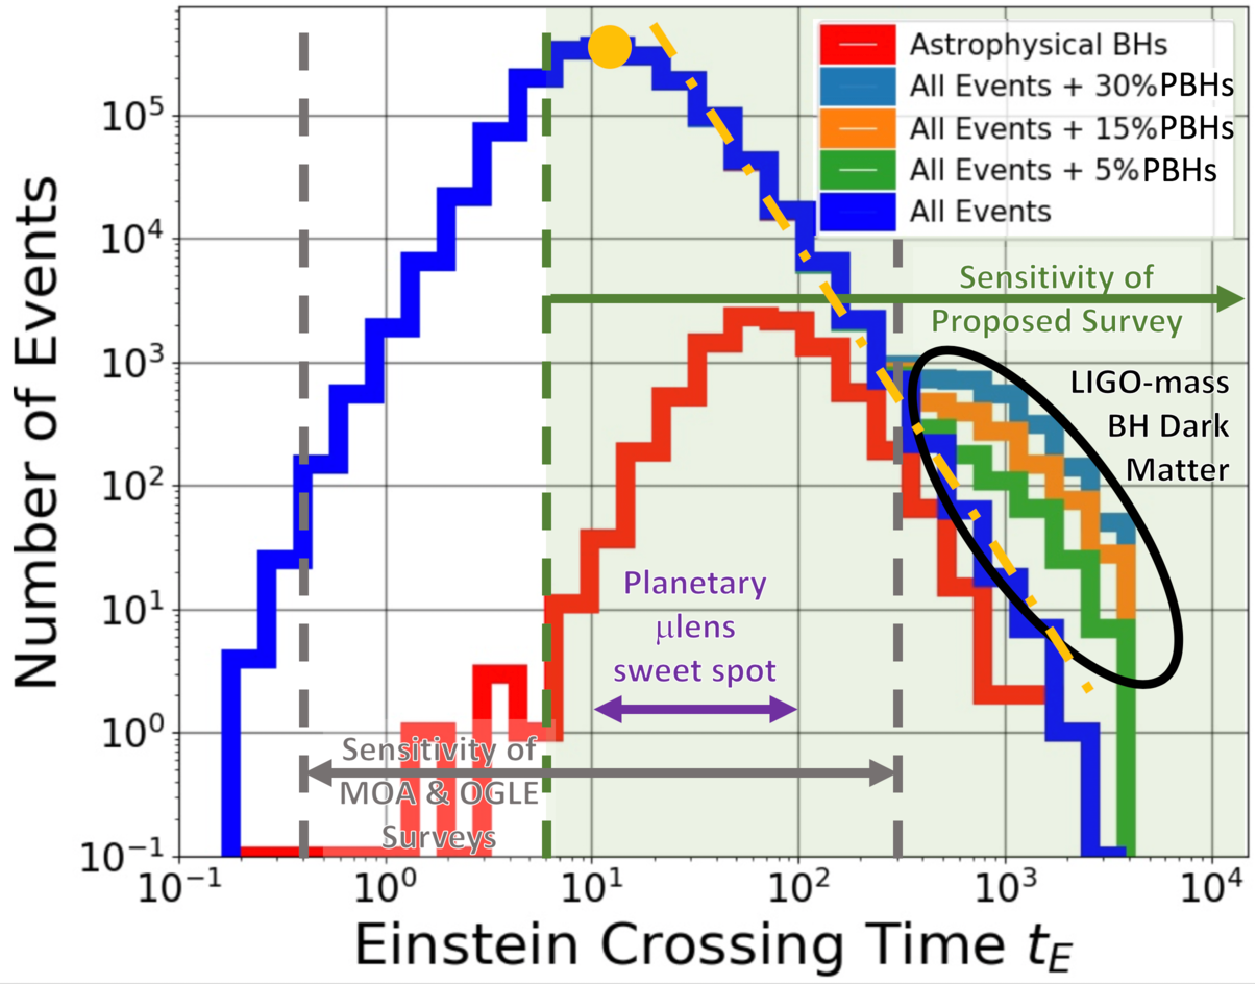
\includegraphics[width=0.6\columnwidth]{nevents_vs_t.pdf}
\caption{
    \label{fig:macho_discovery}
    The expected number of $2\theta_\mathrm{E}$ microlensing events in a $10\times10\,\mathrm{deg}^2$ bulge field (blue histogram), with the fraction due to black holes resulting from stellar evolution shown by the red histogram (for these events our detection efficiency is $\sim0.1\%$ at low-$t_\mathrm{E}$ and $\sim1\%$ at high-$t_\mathrm{E}$).
    \WAD{Need to come up with better estimates for the number of expected event, i.e., how to scale the y-axis for LSST, especially considering different regions of the sky and potentially different cadences in each of these regions. Could just present a conservative estimate for $10\times10\,\mathrm{deg}^2$ bulge field.}
    Other colored histograms show the event rate assuming different fractions of dark matter composed of LIGO-mass black holes (an order of magnitude more massive than the stellar remnant population).
    The gray vertical dashed lines show the published sensitivity ranges of the MOA and OGLE microlensing surveys (insensitive to the high-mass/long-$t_\mathrm{E}$ tail).
    The shaded green regions shows the sensitivity range for LSST.
    %This includes the planetary microlensing sweet spot (purple), which will be probed via alerted follow up.
    It also importantly includes the peak of the distribution (yellow dot), and enables us to accurately calibrate the slope (yellow dot-dashed line), which is necessary to provide accurate IMBH constraints.
    \Contributors{Jessica Lu, Casey Lam, Michael M., Will D.}
    }
\end{figure}

%{\bf SIDM-WDM Discovery}
\subsection{WDM/SIDM Discovery}

We now turn to a more challenging scenario in which dark matter possesses a particle mass or self-interaction cross section that would partially account for observed small-scale structure anomalies.
There are currently several hints of non-minimal dark matter particle properties arising from comparisons between theoretical predictions and observed galaxy populations at the dwarf galaxy scale, i.e., distances below $1 \Mpc$ and mass scales below $10^{11} \Msun$ \citep[reviewed by][]{BuckleyPeter:2017,Bullock:2017xww}.
However, the interpretation of these discrepancies in terms of dark matter microphysics has been hindered by our present uncertainty in the mapping between visible stellar populations and invisible dark matter halos, which involves both the physics of galaxy formation as well as the connection between observable and intrinsic galaxy properties (see \secref{smallest_galaxies} and \secref{halo_profile_group}).
In a regime where we are already limited by systematic uncertainties, it is therefore quite reasonable to ask how the increased statistical power of LSST will help to resolve our current small-scale structure quandary.

We argue here that the decisive advantage of LSST is the opportunity to combine an ensemble of astrophysical dark matter probes that offer complementary perspectives on dark matter halo abundances and profile shapes, and which are affected by different sources of systematic uncertainty.
For the purpose of illustration, we outline a possible ``roadmap to discovery'' for a dark matter model that produces as a cutoff in the matter power spectrum and a suppression of the central dark matter profile just below the current sensitivity limit---i.e., $M_{hm} = 10^{8.5}$.

The first indication of a problem might come shortly after the first public data release of LSST survey data when automated searches for additional Milky Way satellites reveal only a handful of new candidate ultra-faint galaxies. 
Using the framework described in \secref{smallest_galaxies}, these observations could be combined to derive contours on the parameter space of WDM mass vs SIDM cross-section.
As shown in \figref{sidm_wdm_discovery}, there is some degeneracy between WDM particle mass and SIDM cross section.
This degeneracy is reminiscent of similar cosmological contours---e.g., that between $\Omega_m$ and $\sigma_8$.

Using the same LSST data release, the combined depth and sky coverage of LSST will enable the study of dwarf galaxy satellite populations around several other hosts out to several Mpc, as well as the ``field'' population of isolated dwarf galaxies.
By generating a statistical sample of low-luminosity galaxies in a wide variety of environments, LSST will provide a wealth of input data to theoreticians developing galaxy formation simulations.
\FIXME{These observations would help to break degeneracies of reionization physics, stellar feedback internal to the dwarf, etc.}
\FIXME{Targets for spectroscopic follow-up}

In parallel with the study of visible galaxy populations, LSST is expected to reveal many new stellar streams and gravitational lens systems which would provide access to dark matter halos below the mass threshold of galaxy formation \FIXME{add secrefs}.
In our scenario with a halo mass cutoff at the ultra-faint galaxy scale, the search for stream gaps and lensing anomalies would be particularly well motivated.
We could expect a period of several years to collect and analyze follow-up observations of the most favorable streams and lens systems.

{\bf Semi-quantitative extraction of particle properties}

\begin{figure}
\centering
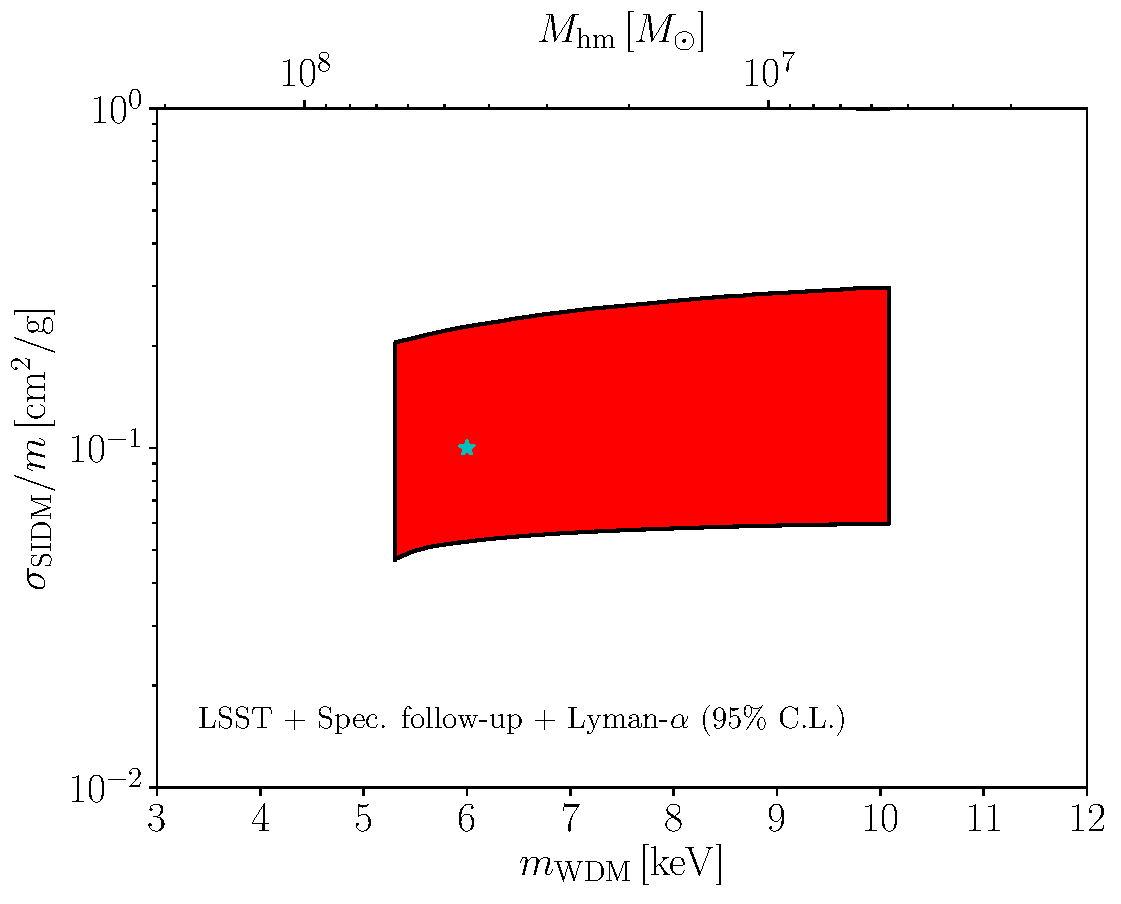
\includegraphics[width=0.6\columnwidth]{figures/SIDM_WDM_fig_disc.pdf}
\caption{\label{fig:sidm_wdm_disc} Potential discovery scenario for particle dark matter. }
\end{figure}

%As a quantitative aspect, we specifically constrain ourselves to the scenario of a dark matter model that manifests itself as a cutoff in the matter power spectrum and a suppression of the central dark matter profile. 

%We assume a maximal model where that cutoff occurs just below the current sensitivity limit---i.e., $M_{hm} = 10^{8.5}$.
%This model would manifest itself as an absence of low-mass dark matter halos detectable through measurements of Milky Way satellites, the lack of gaps in stellar streams, and an underabundance of perturbations in strongly lensed systems.

This is the contour figure from Francis-Yan.

{\bf Roadmap to measurement}

LSST---alone and in synergy with other observations---will deliver a huge leap in sensitivity to dark matter microphysics, through a variety of probes, as discussed previously in this document. 
This promise of opening a broad new parameter space to detailed exploration implies that a discovery of new physics is a real possibility with arrival of the new data. 
We now discuss a road map from detecting anomalous signals, that misalign with the minimal CDM model, to establishing a discovery and measuring particle properties of dark matter.

Anomalies in various data sets were previously tentatively attributed to new dark matter physics, but have so far never risen to a status of a confirmed discovery. 
The main reason is presence of large systematic effects that may be confused with dark matter signals, stemming from a limited understanding of processes characterizing astrophysical systems and observational biases and systematic errors. 
However, the advent of LSST (and similar surveys) offers means to largely circumvent such issues---access to a wide range of observables that may harbor signals of the same dark matter microphysics, but suffer from different systematic effects. 
Combination of orthogonal information from various probes---and measurement of a consistent signal in several of them---will be essential for establishing a discovery. 

\FIXME{This paragraph is work in progress}: As an illustration, imagine a scenario where future satellite number counts from LSST return evidence for a missing population of low-luminosity objects. 
Such measurement could imply presence of a cutoff in the matter power spectrum (as would be produced, for example, by dark matter self-interactions), but it could, alternatively, be a consequence of a lower limit on the dark matter halo mass that can host a galaxy. 
Another observable: spectroscopic follow-up measurements of the radial density profiles… [\FIXME{VG: someone else should finish this} by telling a story of how the latter measures dark matter only, so it is a direct probe of DM, but may be a lower signal-to-noise measurement; in this case, joint analysis of both observables under the SIDM hypothesis may return conclusive evidence in favor of SIDM vs CDM].

Fully utilizing complementary features of different observables requires a probabilistic inference framework that enables joint analysis of multiple measurements probing the same underlying dark-matter physics. 
Such a likelihood-based framework is already being developed for dark energy studies with LSST data and is commonplace for modern cosmological parameter estimation with data from the cosmic microwave background and current galaxy surveys. 
Recent studies (\FIXME{Nadler et al, Jethwa et al: needs check}) have already begun paving the path towards probabilistic analyses of relevant data sets, with the aim of robustly probing astrophysical parameters of interest. 
Extensions of these analyses to include inference of parameters relevant for underlying dark matter physics are underway, and further work is needed in order to formulate frameworks that include other observables. 

Beyond enabling consistent inclusion of all available information and boosting statistical significance of individual measurements, joint likelihood analyses provide a framework for robustly including systematic effects and breaking degeneracy between them and dark matter signals. 
As illustrated in the above example, a marginal discrepancy with CDM in two complementary observables may amount to high-significance detection that highly favors new physics. 
If such analysis includes a generous marginalization over all relevant systematic effects, and if the fit of particular non-minimal dark matter model to \textit{all} observables is vastly better than that of CDM, we will be compelled to claim discovery of dark matter. 
Finally, as we have shown in Section \FIXME{XX} on the example of WDM and SIDM, signals of some theoretical scenarios can be partly degenerate with each other; quantifying this degeneracy, within a statistical parameter estimation framework, will be essential approach for detailed dark matter studies in a post-discovery era.

%In the regime where a ``discovery'' occurs, it is important to examine what ``measurement'' looks like in the context of astrophysical probes with LSST.
%%Using the framework described in \secref{smallest_galaxies}, these observations could be combined to derive contours on the parameter space of WDM mass vs SIDM cross-section.
%%As shown in \figref{sidm_wdm_discovery}, there is some degeneracy between WDM particle mass and SIDM cross section.
%%This degeneracy is reminiscent of similar cosmological contours---e.g., that between $\Omega_m$ and $\sigma_8$.

%Similar to cosmological constraints on dark energy, degeneracies in the fundamental properties of dark matter can be broken through the combination of multiple probes.
%In the simple WDM case of our example, combining measurements from galaxy cluster profiles will help to constrain the SIDM cross section at a scale that is impossible to probe with dwarf galaxies. 

%In the LSST era, dark matter science needs to move from a disperate set of communities of 

\begin{comment}
%ADW: This comment block contains notes from our discussion at Livermore.
\begin{enumerate}
    \item We may start by alluding to the brief era where we thought that neutrinos could have been dark matter before it was proven that they would free stream
    \item This was orthogonal to DOE's mantra: "we don't care where the dark matter is, but what it is"
\end{enumerate}

\begin{enumerate}
    \item Individual analyses can proceed in parallel, just need to be able to create a likelihood
    \item This is the case with the CMB analyses
    \item The dwarf galaxy analysis could be used as a demonstration of one of these likelihoods
\end{enumerate}

\begin{enumerate}
    \item Do we need a specific example of a discovery?
    \item If there was a cutoff at a mass of $10^8 \Msun$, what would it look like?
    \item Can we make an example of the WDM-SIDM figure a closed contour plot?
    \item Make the ``optimistic'' assumption of detecting $10^5 \Msun$ halos.
    \item Assume a cutoff in the mass function at $10^7 \Msun$ (probably not sensitive currently)
    \item Once we have the detection, start expanding to a .
    \item Uncertainties could be wrong, but they will be narrowed down.
    \item In the future we can also include correlations with other parameters
\end{enumerate}

\begin{enumerate}
    \item It is likely premature to assume that are current tools are the only tools that we will have after LSST discoveries
    \item There will likely be new probes and new ways forward.
    \item The dimensionality could be much higher.
    \item Correlation between dark energy and dark matter might explore new models, hitherto unconsidered
    \item Discovery potential for compact object dark matter?
    \item Discovery potential emergent dark matter
\end{enumerate}
\end{comment}
% ----------------------------------------------------------------------
